\chapter*{MEMORIA DESCRIPTIVA}
\addcontentsline{toc}{chapter}{MEMORIA DESCRIPTIVA}

\section{GENERALIDADES}

\subsection{DESCRIPCION}

La presente memoria descriptiva corresponde al proyecto de Instalaciones Electricas Interiores de la vivienda unifamiliar de Aquiles Taylor Ramos Yapo, ubicada en el distrito de San Miguel, provincia de San Roman, departamento de Puno.

El proyecto comprende la descripcion tecnica del sistema electrico interior en baja tension, desde el medidor de energia hasta los tableros, alimentadores, circuitos derivados, salidas de alumbrado, tomacorrientes, cargas especiales y sistema de puesta a tierra. La distribucion arquitectonica empleada como base corresponde a los croquis de la vivienda y a los planos arquitectonicos CAD v3 desarrollados para el primer y segundo piso.

Para efectos de dimensionamiento se adopta el escenario conservador desarrollado en el Capitulo 2: vivienda monofasica de 220 V, cocina electrica considerada como carga especial, lavadora, bomba de agua exterior de 1 HP, alumbrado LED y tomacorrientes con conductor de proteccion. Los valores adoptados no eliminan la obligacion de verificar en obra la ubicacion final de equipos, pero permiten cerrar la memoria con criterios electricos coherentes y reglamentarios.

\subsection{NOMBRE DEL PROYECTO}

La presente memoria descriptiva corresponde a la elaboracion del expediente academico del Proyecto:

\begin{quote}
\textbf{``INSTALACIONES ELECTRICAS INTERIORES DE VIVIENDA UNIFAMILIAR, DISTRITO DE SAN MIGUEL -- PROVINCIA DE SAN ROMAN -- DEPARTAMENTO DE PUNO''.}
\end{quote}

\subsection{UBICACION}

El proyecto se encuentra ubicado en:

\begin{center}
\begin{tabular}{p{1.45in}c p{3.20in}}
Region & : & Puno \\
Provincia & : & San Roman \\
Distrito & : & San Miguel \\
Referencia & : & Avenida Horacio con Jr. Marineros, manzana F7, lotes 11 y 12 \\
Zona & : & Urbana \\
\end{tabular}
\end{center}

La ubicacion geografica del proyecto se representa de forma secuencial desde el departamento de Puno, la provincia de San Roman y el distrito de San Miguel, donde se desarrolla la vivienda materia del presente expediente.

\begin{figure}[H]
\centering

\includegraphics[width=0.32\textwidth]{figuras/mapa-01-departamento-puno.png}
\hfill

\includegraphics[width=0.58\textwidth]{figuras/mapa-02-provincia-san-roman.png}
\par\vspace{1.0em}
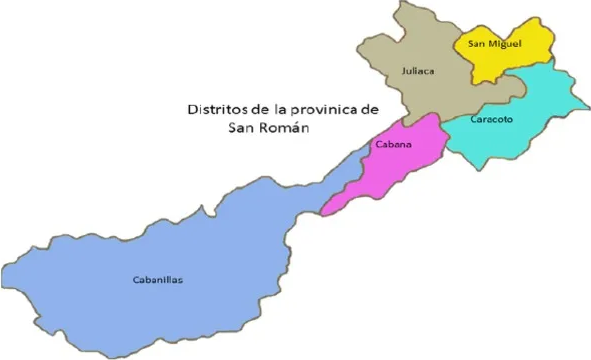
\includegraphics[width=0.58\textwidth]{figuras/mapa-03-distrito-san-miguel.png}
\caption{Ubicacion geografica del proyecto: departamento de Puno (arriba izquierda), provincia de San Roman (arriba derecha) y distrito de San Miguel (abajo).}
\end{figure}

\begin{figure}[H]
\centering
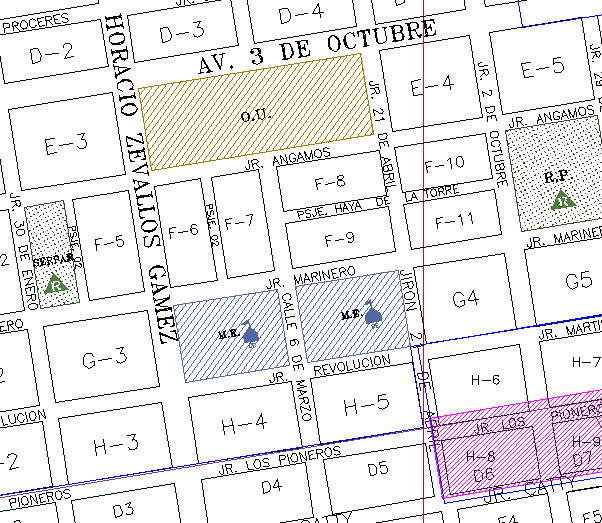
\includegraphics[width=0.70\textwidth]{figuras/catastro-aquiles.png}
\caption{Referencia catastral de la zona de ubicacion de la vivienda.}
\end{figure}

\subsubsection{CONDICIONES CLIMATOLOGICAS}

La zona del proyecto corresponde al ambito urbano altoandino del departamento de Puno, en el distrito de San Miguel, a una altitud promedio de \textbf{3,825 m.s.n.m.} La topografia es predominantemente plana. Para el diseno electrico se consideran las condiciones ambientales de la region, resumidas en la siguiente tabla (fuente de informacion climatologica: SENAMHI / TuTiempo.net):

\begin{center}
\begin{small}
\begin{tabular}{l c c}
\toprule
\textbf{Parametro climatologico} & \textbf{Mayo - octubre} & \textbf{Noviembre - abril} \\
\midrule
Clima predominante & Frigido y seco & Frigido y lluvioso \\
Temperatura minima & \(-3^\circ\text{C}\) & \(0^\circ\text{C}\) \\
Temperatura maxima & \(17^\circ\text{C}\) & \(19^\circ\text{C}\) \\
Temperatura media & \(8^\circ\text{C}\) & \(14^\circ\text{C}\) \\
Velocidad del viento & 90 km/h & 70 km/h \\
\bottomrule
\end{tabular}
\end{small}
\end{center}

Las bajas temperaturas y lluvias estacionales se consideran para la seleccion de cubiertas aislantes, cajas exteriores, canalizaciones enterradas y accesorios resistentes a humedad.

\subsubsection{DATOS DE COORDENADAS}

Las coordenadas geograficas de referencia para la vivienda unifamiliar son:

\begin{center}
\begin{tabular}{p{2.20in}c p{2.65in}}
Coordenadas del predio & : & -15.46546784841618, -70.13460258266534 \\
\end{tabular}
\end{center}

\subsection{OBJETIVOS}

\subsubsection{OBJETIVO GENERAL}

Satisfacer las necesidades de energia electrica de la vivienda unifamiliar de dos pisos mediante una instalacion interior segura, funcional, mantenible y compatible con la distribucion arquitectonica levantada en los planos CAD del proyecto.

\subsubsection{OBJETIVOS ESPECIFICOS}

\begin{itemize}
  \item Establecer el sistema de alimentacion principal, tableros, alimentaciones secundarias y circuitos derivados de la vivienda.
  \item Definir la distribucion electrica para alumbrado, tomacorrientes generales y cargas especiales.
  \item Seleccionar conductores, tuberias, interruptores termomagneticos e interruptores diferenciales de acuerdo con el calculo de demanda, caida de tension y coordinacion electrica.
  \item Incorporar proteccion por puesta a tierra y proteccion diferencial de 30 mA para los circuitos de utilizacion.
  \item Presentar criterios de instalacion empotrada en PVC, cajas, empalmes, colores de conductores, pruebas y simbologia de planos.
\end{itemize}

\subsection{ALCANCES DEL PROYECTO}

El proyecto comprende el diseno de las instalaciones electricas interiores en baja tension para una vivienda unifamiliar de dos niveles. El predio se considera con area de terreno referencial de \(134.18\text{ m}^2\). Para los calculos electricos se adopta un area techada total de referencia de \(120.00\text{ m}^2\), empleada para aplicar la Regla 050-200 del Codigo Nacional de Electricidad -- Utilizacion y contrastar la demanda por area con la demanda por circuitos.

Los componentes principales del sistema son:

\begin{itemize}
  \item Suministro monofasico de 220 V, 60 Hz, desde medidor de energia hacia el Tablero General.
  \item Tablero General (TG) empotrado en el primer piso, ubicado segun el plano electrico del primer nivel.
  \item Alimentacion secundaria hacia tablero de segundo piso (T2), ubicado segun el plano electrico del segundo nivel.
  \item Circuitos derivados C1 a C8 para alumbrado, tomacorrientes, cocina electrica, lavadora y bomba exterior.
  \item Canalizaciones interiores empotradas en muros y losas con tuberia PVC-P.
  \item Canalizacion subterranea protegida para la bomba de agua exterior.
  \item Conductores de cobre con aislamiento termoplastico no propagador de llama, identificados por colores normalizados.
  \item Sistema de puesta a tierra con barra de tierra en tableros y conductor de proteccion hacia todas las salidas con contacto a tierra.
\end{itemize}

\subsection{NORMAS DE APLICACION}

El proyecto se desarrolla bajo los requisitos tecnicos de las normas nacionales aplicables a instalaciones electricas interiores:

\begin{itemize}
  \item Codigo Nacional de Electricidad -- Utilizacion, aprobado por RM N\(^\circ\) 0037-2006-MEM/DM.
  \item Reglamento Nacional de Edificaciones, Norma EM.010 Instalaciones Electricas Interiores.
  \item Norma DGE ``Simbolos Graficos en Electricidad'', RM N\(^\circ\) 091-2002-EM/VME.
  \item Normas Tecnicas Peruanas aplicables a tuberias PVC, cajas, conductores, tomacorrientes, interruptores y accesorios.
  \item Criterios de conexion, medicion y acometida de la empresa concesionaria Electro Puno S.A.A.
  \item Sistema Legal de Unidades de Medida del Peru.
\end{itemize}

En caso de diferencia entre una practica de obra y una exigencia normativa, prevalece la exigencia del Codigo Nacional de Electricidad -- Utilizacion y de la Norma EM.010.

\section{DESCRIPCION DEL PROYECTO}

\subsection{ALIMENTADORES PRINCIPALES}

El alimentador principal suministra energia desde el medidor de la concesionaria hasta el Tablero General de la vivienda. El recorrido se proyecta lo mas directo posible, protegido mecanicamente y con conductor de proteccion incluido.

De acuerdo con el calculo justificativo, la maxima demanda adoptada para el escenario conservador es \textbf{10,358 W}. Con tension monofasica de 220 V y factor de potencia 0.90, se obtiene una corriente de empleo de \textbf{52.31 A} y una corriente de diseno de \textbf{65.39 A}. Por ello se adopta alimentador de \textbf{2 conductores activos de cobre de 16 mm$^2$ + conductor de proteccion de 10 mm$^2$}, instalado en tuberia PVC-P de \textbf{40 mm}. La proteccion general se realiza mediante interruptor termomagnetico bipolar de \textbf{63 A}.

La caida de tension calculada para el alimentador es \textbf{0.635 \%}, por debajo del limite de referencia de 2.5 \% para alimentadores y del limite total de 4.0 \% establecido como criterio de diseno en el CNE-U.

\subsection{TABLERO ELECTRICO GENERAL}

El Tablero General (TG) sera empotrado en el primer piso, en la zona indicada en el plano electrico del primer nivel, cerca del acceso y proximo al medidor. Esta ubicacion facilita maniobra, mantenimiento, lectura de protecciones y reduccion del recorrido medidor--tablero.

El tablero sera metalico, con puerta, riel DIN, barra de neutro aislada, barra de tierra y espacio suficiente para interruptor general, interruptores diferenciales y circuitos derivados. El interruptor general sera \textbf{2P-63 A}. Desde el TG se atenderan los circuitos del primer piso y se derivara la alimentacion secundaria hacia el tablero de segundo piso (T2).

El gabinete debera instalarse empotrado en muro, con frente accesible, rotulado de circuitos, identificacion de barras y reserva fisica minima para futuras ampliaciones razonables. No se admiten conexiones sueltas ni empalmes internos fuera de borneras o barras adecuadas.

\subsection{ALIMENTADORES SECUNDARIOS}

La vivienda contara con una alimentacion secundaria desde el TG hacia el tablero del segundo piso (T2). El T2 aparece en el plano electrico del segundo nivel y concentra los circuitos C4, C5, C6 y C7, reduciendo recorridos de canalizacion y facilitando el mantenimiento por piso.

Para esta alimentacion secundaria se adopta conductor de cobre \textbf{2 x 16 mm$^2$ + PE 10 mm$^2$}, en tuberia PVC-P de \textbf{40 mm}, protegido desde el TG mediante interruptor termomagnetico bipolar de \textbf{50 A}. En el T2 se instalaran los dispositivos de proteccion de alumbrado, tomacorrientes, cocina electrica y lavadora del segundo nivel.

\subsubsection{CANALIZACIONES}

Las canalizaciones interiores seran empotradas en muros, losas y elementos de concreto o ladrillo. Se empleara tuberia de PVC rigido clase pesada (PVC-P), retardante de llama, con diametros de 20 mm para circuitos derivados generales, 32 mm para la cocina electrica y 40 mm para alimentadores.

No se proyectan instalaciones aparentes ni ductos sobresalientes en paredes interiores. Las bajadas a interruptores y tomacorrientes se ejecutaran dentro de muro, conectadas a cajas rectangulares embutidas. Las salidas de techo se ejecutaran con cajas octogonales y las derivaciones mediante cajas de paso registrables.

Para el circuito C8 de bomba de agua exterior se admite canalizacion subterranea en PVC-P, instalada en zanja protegida, con cama de material fino, cubierta mecanica y cinta de advertencia. Las cajas o buzones empotrados exteriores se ubicaran solo donde sea necesario para inspeccion y mantenimiento.

\subsubsection{CABLES ALIMENTADORES}

Los cables alimentadores y derivados seran de cobre electrolitico, aislamiento termoplastico para 450/750 V o superior segun disponibilidad comercial, no propagadores de llama y aptos para instalacion en tuberia empotrada. En zonas con mayor exigencia de seguridad se preferiran conductores libres de halogenos y de baja emision de humos.

Los conductores seran instalados continuos de caja a caja o de tablero a caja, sin empalmes dentro de tuberias. El tendido se realizara con guiado adecuado, evitando aceite, grasa u otro material que deteriore el aislamiento.

\begin{table}[H]
\centering
\small
\caption{Conductores, tuberias y protecciones adoptadas}
\resizebox{\textwidth}{!}{%
\begin{tabular}{l p{3.0cm} p{3.3cm} p{2.0cm} p{2.0cm} p{2.6cm}}
\toprule
\textbf{Circuito} & \textbf{Servicio} & \textbf{Conductores} & \textbf{Tuberia} & \textbf{ITM} & \textbf{Proteccion diferencial} \\
\midrule
Alim. TG & Medidor a TG & 2 x 16 mm$^2$ Cu + PE 10 mm$^2$ & PVC-P 40 mm & 2P-63 A & Diferencial general/selectivo segun tablero \\
Alim. T2 & TG a tablero segundo piso & 2 x 16 mm$^2$ Cu + PE 10 mm$^2$ & PVC-P 40 mm & 2P-50 A & En tablero T2 por grupos de circuitos \\
C1 & Alumbrado primer piso & 2 x 2.5 mm$^2$ Cu + PE 2.5 mm$^2$ & PVC-P 20 mm & 2P-10 A & ID 2P-25 A, 30 mA \\
C2 & Tomacorrientes primer piso & 2 x 2.5 mm$^2$ Cu + PE 2.5 mm$^2$ & PVC-P 20 mm & 2P-10 A & ID 2P-25 A, 30 mA \\
C3 & Toma auxiliar cocina primer piso & 2 x 2.5 mm$^2$ Cu + PE 2.5 mm$^2$ & PVC-P 20 mm & 2P-10 A & ID 2P-25 A, 30 mA \\
C4 & Alumbrado segundo piso & 2 x 2.5 mm$^2$ Cu + PE 2.5 mm$^2$ & PVC-P 20 mm & 2P-10 A & ID 2P-25 A, 30 mA \\
C5 & Tomacorrientes segundo piso & 2 x 2.5 mm$^2$ Cu + PE 2.5 mm$^2$ & PVC-P 20 mm & 2P-10 A & ID 2P-25 A, 30 mA \\
C6 & Cocina electrica segundo piso & 2 x 10 mm$^2$ Cu + PE 10 mm$^2$ & PVC-P 32 mm & 2P-32 A & ID 2P-40 A, 30 mA \\
C7 & Lavadora segundo piso & 2 x 2.5 mm$^2$ Cu + PE 2.5 mm$^2$ & PVC-P 20 mm & 2P-10 A & ID 2P-25 A, 30 mA \\
C8 & Bomba de agua exterior & 2 x 2.5 mm$^2$ Cu + PE 2.5 mm$^2$ & PVC-P 20 mm & 2P-10 A & ID 2P-25 A, 30 mA \\
\bottomrule
\end{tabular}%
}
\end{table}

\subsubsection{UNIONES Y EMPALMES DE CONDUCTORES}

Las uniones y empalmes se ejecutaran unicamente dentro de cajas de paso, cajas de salida o tableros, quedando siempre accesibles para inspeccion. Cada empalme debera asegurar continuidad electrica, resistencia mecanica y aislamiento equivalente al conductor original.

Se emplearan conectores aislados, borneras, terminales o conectores de cobre adecuados a la seccion del conductor. Donde se utilice cinta aislante, esta sera de buena calidad, autoadhesiva, resistente a la humedad, con rigidez dielectrica suficiente para baja tension y aplicada en capas continuas que cubran completamente la union.

\subsubsection{UNIONES Y EMPALMES DENTRO DE CANALIZACIONES}

Quedan prohibidos los empalmes dentro de tuberias, curvas, conectores o tramos cerrados de canalizacion. Todo conductor que recorra una tuberia debera pasar libremente y sin uniones internas. Las derivaciones se haran solamente en cajas registrables.

\subsection{TABLEROS ELECTRICOS DE DISTRIBUCION}

El sistema tendra dos tableros principales de distribucion interior:

\begin{itemize}
  \item \textbf{TG - Primer piso:} recibe el alimentador desde medidor, contiene el interruptor general de 63 A, proteccion de los circuitos del primer piso, salida al tablero T2 y circuito de bomba exterior.
  \item \textbf{T2 - Segundo piso:} recibe la alimentacion secundaria desde el TG y protege los circuitos de alumbrado, tomacorrientes, cocina electrica y lavadora del segundo nivel.
\end{itemize}

Ambos tableros seran empotrados, metalicos, con tapa, riel DIN, borneras, barras de neutro y tierra, rotulado permanente de circuitos y espacio de reserva. La disposicion interna debera permitir que el conductor de proteccion nunca sea interrumpido por interruptores o seccionadores.

\subsubsection{INTERRUPTORES TERMOMAGNETICOS}

Los interruptores termomagneticos seran bipolares, montados sobre riel DIN, con accionamiento manual y disparo automatico por sobrecarga y cortocircuito. La corriente nominal del interruptor se selecciona cumpliendo el criterio de coordinacion:

\[
I_b \leq I_n \leq I_z
\]

donde \(I_b\) es la corriente de empleo, \(I_n\) la corriente nominal del interruptor e \(I_z\) la capacidad de conduccion del conductor. Bajo este criterio, el alimentador principal queda protegido por ITM 2P-63 A y los circuitos derivados generales por ITM 2P-10 A. La cocina electrica C6 requiere ITM 2P-32 A por su mayor corriente de empleo.

\subsubsection{INTERRUPTORES DIFERENCIALES}

Los interruptores diferenciales seran de alta sensibilidad, con corriente residual nominal de \textbf{30 mA}, instalados aguas abajo de los termomagneticos correspondientes o agrupando circuitos compatibles. Su uso responde al criterio de proteccion de personas contra contactos indirectos y corrientes de fuga, sin reemplazar el sistema de puesta a tierra.

Se adopta proteccion diferencial para circuitos de tomacorrientes, cocina, lavadora, bomba exterior y alumbrado. Para C6 se emplea diferencial de 40 A, 30 mA; para los demas grupos se emplean diferenciales de 25 A, 30 mA, coordinados con los interruptores de 10 A.

\subsection{CIRCUITOS DERIVADOS}

Los circuitos derivados se distribuyen de acuerdo con los planos electricos del proyecto y el cuadro de cargas calculado:

\begin{itemize}
  \item C1: alumbrado del primer piso.
  \item C2: tomacorrientes generales del primer piso.
  \item C3: tomacorriente auxiliar de cocina del primer piso.
  \item C4: alumbrado del segundo piso.
  \item C5: tomacorrientes generales del segundo piso.
  \item C6: cocina electrica o carga especial de cocina del segundo piso.
  \item C7: lavadora del segundo piso.
  \item C8: bomba de agua exterior.
\end{itemize}

Todos los circuitos incluyen conductor de proteccion a tierra. La instalacion se ejecutara empotrada en paredes y techos con tuberia PVC-P, saliendo a cajas normalizadas para luminarias, interruptores, tomacorrientes y equipos.

\subsubsection{TUBOS DE PLASTICO PVC}

Se utilizaran tubos de plastico PVC rigido pesado. Para circuitos derivados de alumbrado y tomacorrientes se adopta diametro minimo de 20 mm; para la cocina electrica C6 se adopta 32 mm; para los alimentadores principal y secundario se adopta 40 mm.

Las curvas seran amplias y comerciales, evitando radios cerrados que dificulten el cableado. No se aceptaran aplastamientos, empalmes improvisados de tubo ni tramos sin continuidad mecanica entre caja y caja.

\subsubsection{TUBOS METALICOS}

No se proyectan tubos metalicos para canalizaciones generales. La instalacion residencial se ejecutara con PVC empotrado. Los elementos metalicos previstos corresponden a cajas, tableros, tapas y accesorios donde resulte necesario por resistencia mecanica o presentacion.

\subsubsection{SOPORTES Y ACCESORIOS}

Las cajas y tuberias se fijaran antes del tarrajeo o vaciado, manteniendo nivel, alineamiento y profundidad adecuada. Las tuberias llegaran a las cajas mediante conectores; no se permitira que el tubo quede simplemente apoyado o suelto dentro del muro.

Para salidas de tomacorriente e interruptores se emplearan cajas rectangulares embutidas. Para salidas de luminarias se emplearan cajas octogonales. En derivaciones o cambios de ruta se emplearan cajas cuadradas de paso con tapa.

\subsubsection{CAJAS PARA SALIDAS}

Las cajas de salida seran de fierro galvanizado pesado o material normalizado equivalente. Las cajas para interruptores y tomacorrientes seran rectangulares; las de luminarias, octogonales; y las de paso, cuadradas con tapa desmontable.

Las cajas quedaran al ras del acabado final del muro o cielo raso. No se admiten cajas hundidas excesivamente ni cajas sobresalientes que generen riesgo mecanico o mala presentacion. Los bordes se mantendran limpios para permitir el montaje correcto de placas, luminarias y accesorios.

\subsubsection{CAJAS METALICAS PARA TABLEROS}

El Tablero General del primer piso y el tablero T2 del segundo piso se instalaran en cajas metalicas empotradas. Estas cajas tendran tapa, bisagra o sistema de cierre, placa interna para equipos DIN, conexion a tierra de la envolvente y espacio suficiente para cableado ordenado.

Las entradas de tuberia al tablero deberan conservar proteccion mecanica, sin aristas cortantes y con identificacion clara de alimentadores y circuitos.

\subsubsection{CAJAS DE PASO}

Las cajas de paso se instalaran en tramos donde el recorrido, cantidad de curvas o cambio de direccion lo requiera. En exteriores o tramos subterraneos se emplearan cajas o buzones empotrados, protegidos contra humedad y con tapa registrable.

\subsubsection{CINTA AISLANTE Y ACCESORIOS DE EMPALME}

La cinta aislante sera para uso electrico en baja tension, resistente a humedad y temperatura normal de servicio, con rigidez dielectrica adecuada. Su aplicacion no sustituye conectores mecanicos: primero se asegura la union con conector o bornera y luego se restituye el aislamiento.

\subsection{ILUMINACION GENERAL}

La iluminacion se resuelve mediante luminarias LED de alta eficiencia, ubicadas segun los planos electricos de cada piso. Para el calculo manual se emplea el metodo de los lumenes:

\[
E = \frac{N \cdot \Phi \cdot CU \cdot FM}{A}
\]

donde \(E\) es la iluminancia media en lux, \(N\) el numero de luminarias, \(\Phi\) el flujo luminoso minimo por luminaria, \(CU\) el coeficiente de utilizacion, \(FM\) el factor de mantenimiento y \(A\) el area del ambiente. Se adopta \(\Phi = 3000\text{ lm}\), \(CU = 0.75\) y \(FM = 0.90\), por tratarse de luminarias LED de distribucion general en ambientes residenciales.

\subsubsection{NIVEL DE ILUMINACION}

Los niveles minimos se toman de la Norma EM.010 y de criterios usuales para vivienda: escaleras 150 lux, pasadizos y banos 100 lux, cocina 300 lux, ambientes de permanencia 50 a 100 lux segun uso.

\begin{table}[H]
\centering
\scriptsize
\caption{Verificacion manual de iluminacion por ambiente}
\resizebox{\textwidth}{!}{%
\begin{tabular}{l l r r r r l}
\toprule
\textbf{Piso} & \textbf{Ambiente} & \textbf{Area (m$^2$)} & \textbf{Luminarias} & \textbf{Lux calculado} & \textbf{Lux requerido} & \textbf{Estado} \\
\midrule
1 & Escalera & 13.50 & 1 & 150 & 150 & Cumple \\
1 & Ambiente superior 1 & 27.00 & 1 & 75 & 50 & Cumple \\
1 & Ambiente superior 2 & 27.00 & 1 & 75 & 50 & Cumple \\
1 & Garaje techado & 36.00 & 1 & 56 & 50 & Cumple \\
2 & Escalera & 13.50 & 1 & 150 & 150 & Cumple \\
2 & Cocina grande & 13.50 & 2 & 300 & 300 & Cumple \\
2 & Oficina / varios & 13.50 & 1 & 150 & 100 & Cumple \\
2 & Cuarto superior & 13.50 & 1 & 150 & 50 & Cumple \\
2 & Sala & 13.50 & 2 & 300 & 100 & Cumple \\
2 & Pasadizo y hall & 13.50 & 1 & 150 & 100 & Cumple \\
2 & Bano & 4.50 & 1 & 450 & 100 & Cumple \\
2 & Cuarto inferior en L & 21.30 & 2 & 190 & 50 & Cumple \\
\bottomrule
\end{tabular}%
}
\end{table}

El resultado confirma que la cantidad de puntos de luz prevista en los planos electricos es suficiente para iluminacion general. La seleccion comercial final de luminarias debera garantizar el flujo minimo indicado por punto.

\subsubsection{TIPOS DE LAMPARAS UTILIZADAS}

Se utilizaran luminarias LED de techo, de bajo consumo, con flujo luminoso suficiente para cumplir la tabla anterior. En cocina y sala se admiten luminarias lineales o de mayor flujo para alcanzar la iluminancia requerida sin incrementar innecesariamente la potencia instalada.

\subsection{TOMACORRIENTES}

Los tomacorrientes seran bipolares con contacto de tierra, tipo Schuko o equivalente normalizado, con placa y caja empotrada. Los tomacorrientes de cocina, bano, lavadora y bomba exterior estaran protegidos diferencialmente.

La distribucion queda resumida de la siguiente forma:

\begin{table}[H]
\centering
\small
\caption{Distribucion de tomacorrientes segun planos electricos y calculos}
\begin{tabularx}{\textwidth}{l l r L}
\toprule
\textbf{Piso} & \textbf{Circuito} & \textbf{Cantidad} & \textbf{Uso} \\
\midrule
1 & C2 & 7 & Tomacorrientes generales del primer piso, ambientes superiores y garaje techado. \\
1 & C3 & 1 & Tomacorriente auxiliar de cocina bajo escalera. \\
1 & C8 & 1 & Salida dedicada para bomba de agua exterior. \\
2 & C5 & 12 & Tomacorrientes generales del segundo piso y toma protegida en bano. \\
2 & C6 & 3 & Tomas de cocina electrica y servicio de cocina. \\
2 & C7 & 1 & Salida dedicada para lavadora. \\
\bottomrule
\end{tabularx}
\end{table}

La cantidad total considerada para calculo es de \textbf{25 salidas de tomacorriente o carga puntual}, incluyendo cargas dedicadas de cocina, lavadora y bomba.

\subsection{SISTEMA DE PUESTA A TIERRA}

El proyecto considera Sistema de Puesta a Tierra (S.P.A.T.) para proteccion de personas, continuidad de masas metalicas y operacion adecuada de interruptores diferenciales. El sistema estara formado por pozo de tierra vertical, electrodo de cobre, conductor de puesta a tierra, caja de registro, barra de tierra en TG y barra de tierra en T2.

El conductor de proteccion acompana a todos los alimentadores y circuitos derivados. Para el alimentador general y la alimentacion al T2 se adopta PE de \textbf{10 mm$^2$}; para circuitos derivados generales, PE de \textbf{2.5 mm$^2$}; para C6, PE de \textbf{10 mm$^2$}. La resistencia objetivo del sistema de puesta a tierra sera no mayor a \textbf{25 ohm}, verificable con telurimetro. Si el ensayo arroja un valor superior, se mejorara el sistema con tratamiento de suelo o electrodo adicional.

El pozo de tierra y la ruta del conductor PE deben incorporarse graficamente en los planos electricos finales, ya que forman parte del sistema de seguridad de la instalacion.

\subsection{COLORES EN LOS CONDUCTORES}

La identificacion de conductores se ejecutara de acuerdo con la Regla 030-036 del CNE-U:

\begin{itemize}
  \item Conductores activos en sistema monofasico: negro y rojo.
  \item Conductor neutro o conductor identificado puesto a tierra: blanco.
  \item Conductor de proteccion a tierra: verde o verde con franja amarilla.
\end{itemize}

El color verde o verde/amarillo se reserva exclusivamente para conductor de proteccion. No se permitira usarlo como fase, retorno o conductor de mando.

\subsection{PRUEBAS ELECTRICAS}

Antes de energizar la instalacion se ejecutaran pruebas de continuidad, polaridad, aislamiento y puesta a tierra. Las pruebas se realizaran con todos los interruptores cerrados, equipos desconectados y circuitos identificados.

\subsubsection{PRUEBAS DE AISLAMIENTO}

La resistencia de aislamiento se medira entre conductores activos y entre conductores activos y tierra, empleando megohmetro de tension adecuada para instalaciones de baja tension. Los valores obtenidos deberan cumplir los limites minimos establecidos por el CNE-U para circuitos residenciales.

Tambien se verificara continuidad del conductor de proteccion, disparo de interruptores diferenciales mediante boton de prueba y ausencia de conexion accidental entre neutro y tierra aguas abajo de los diferenciales.

\subsection{SIMBOLOS}

La simbologia de los planos electricos se basa en la Norma DGE ``Simbolos Graficos en Electricidad'', RM N\(^\circ\) 091-2002-EM/VME, Seccion 9, Instalaciones en Edificios. Los simbolos de luminaria, interruptor, tomacorriente, tablero, medidor, puesta a tierra y canalizacion deberan conservarse uniformes en todos los planos.

\subsection{CUADRO DE CARGAS Y MAXIMA DEMANDA}

El cuadro de cargas se toma del Capitulo 2 de Calculos Justificativos. Para la memoria se resume la demanda adoptada por circuitos, considerando el escenario conservador con cocina electrica.

\begin{table}[H]
\centering
\scriptsize
\caption{Cuadro resumen de cargas y maxima demanda}
\resizebox{\textwidth}{!}{%
\begin{tabular}{l p{4.2cm} r r r r l}
\toprule
\textbf{Circuito} & \textbf{Descripcion} & \textbf{P. instalada (W)} & \textbf{F.D.} & \textbf{M.D. (W)} & \textbf{Ib (A)} & \textbf{Proteccion} \\
\midrule
C1 & Alumbrado primer piso & 80 & 1.00 & 80 & 0.40 & 2P-10 A \\
C2 & Tomacorrientes primer piso & 1,260 & 0.70 & 882 & 4.46 & 2P-10 A \\
C3 & Cocina auxiliar primer piso & 300 & 0.80 & 240 & 1.21 & 2P-10 A \\
C4 & Alumbrado segundo piso & 132 & 1.00 & 132 & 0.67 & 2P-10 A \\
C5 & Tomacorrientes segundo piso & 2,340 & 0.70 & 1,638 & 8.27 & 2P-10 A \\
C6 & Cocina electrica segundo piso & 6,000 & 1.00 & 6,000 & 30.30 & 2P-32 A \\
C7 & Lavadora segundo piso & 800 & 0.80 & 640 & 3.23 & 2P-10 A \\
C8 & Bomba de agua exterior & 746 & 1.00 & 746 & 3.77 & 2P-10 A \\
\midrule
\multicolumn{2}{r}{\textbf{Total}} & \textbf{11,658} &  & \textbf{10,358} & \textbf{52.31} & ITM general 2P-63 A \\
\bottomrule
\end{tabular}%
}
\end{table}

El metodo gobernante es la demanda por circuitos derivados, con maxima demanda adoptada de \textbf{10,358 W}. Este valor es mayor que la demanda minima por area y cocina electrica calculada con la Regla 050-200 del CNE-U para el escenario adoptado, por lo que se utiliza para seleccionar el alimentador, tablero general e interruptor general.
